% !Mode:: "TeX:UTF-8" 



\BiSection{3.6}{Figures}

\fancyhead[R]{本题3.6由QC.Z完成}



解:

$I_D=\frac{1}{2}\mu_nC_{ox}\frac{W}{L}(V_{GS}-V_{TH})^2(1+\lambda V_{DS})$\ding{172}

$g_m=\mu_nC_{ox}\frac{W}{L}(V_{GS}-V_{TH})(1+\lambda V_{DS})$\ding{173}

由\ding{172}有$(1+\lambda V_{DS})=\frac{I_D}{\frac{1}{2}\mu_nC_{ox}\frac{W}{L}(V_{GS}-V_{TH})^2}=\frac{2I_D}{\mu_nC_{ox}\frac{W}{L}(V_{GS}-V_{TH})^2}$\ding{174}

\ding{174}代入\ding{173}得$g_m=\mu_nC_{ox}\frac{W}{L}(V_{GS}-V_{TH})\frac{2I_D}{\mu_nC_{ox}\frac{W}{L}(V_{GS}-V_{TH})^2}=\frac{2I_D}{V_{GS}-V_{TH}}$

$r_o=\frac{1+\lambda V_{DS}}{\lambda I_D}$\textcolor{blue}{(见教材P30的2.47)}

\begin{figure}[H] %H为当前位置,!htb为忽略美学标准,htbp为浮动图形
	\begin{minipage}{\linewidth}
		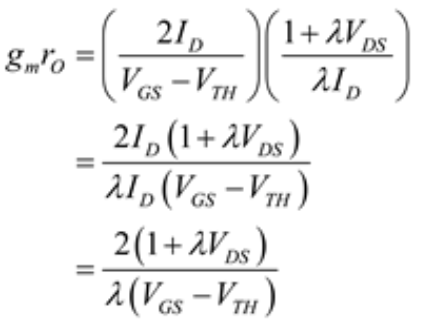
\includegraphics{3.6-1}
	\end{minipage}
\end{figure}

将\ding{174}代入上式得

\begin{figure}[H] %H为当前位置,!htb为忽略美学标准,htbp为浮动图形
	\begin{minipage}{\linewidth}
		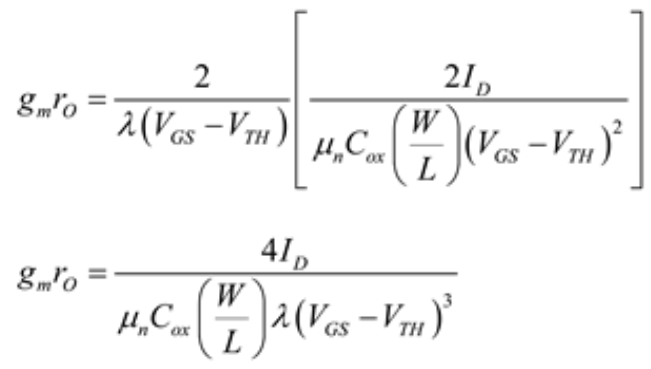
\includegraphics{3.6-2}
	\end{minipage}
\end{figure}

$C_{ox}=\frac{\epsilon_{ox}}{T_{ox}}=\frac{3.9 \times 8.854 \times 10^{-12}\frac{F}{m}}{9 \times 10^{-9}m}=3.837 \times 10^{-3}\frac{F}{m^2}$

\begin{figure}[H] %H为当前位置,!htb为忽略美学标准,htbp为浮动图形
	\begin{minipage}{\linewidth}
		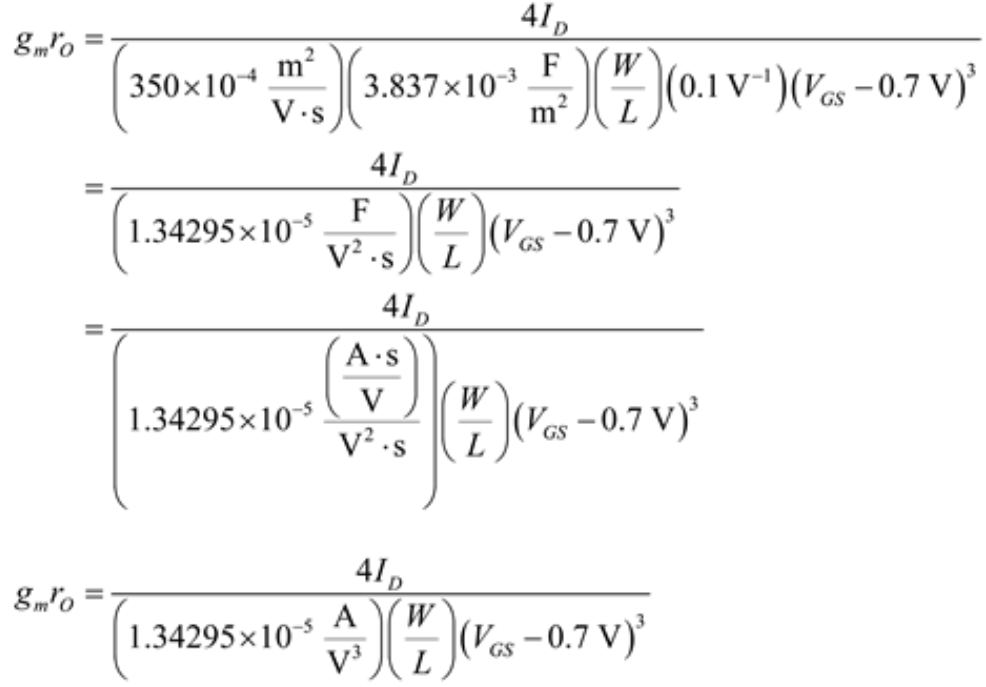
\includegraphics{3.6-3}
	\end{minipage}
\end{figure}

\scalebox{3}{(a)}

		\begin{figure}[H] %H为当前位置,!htb为忽略美学标准,htbp为浮动图形
	\begin{minipage}{\linewidth}
		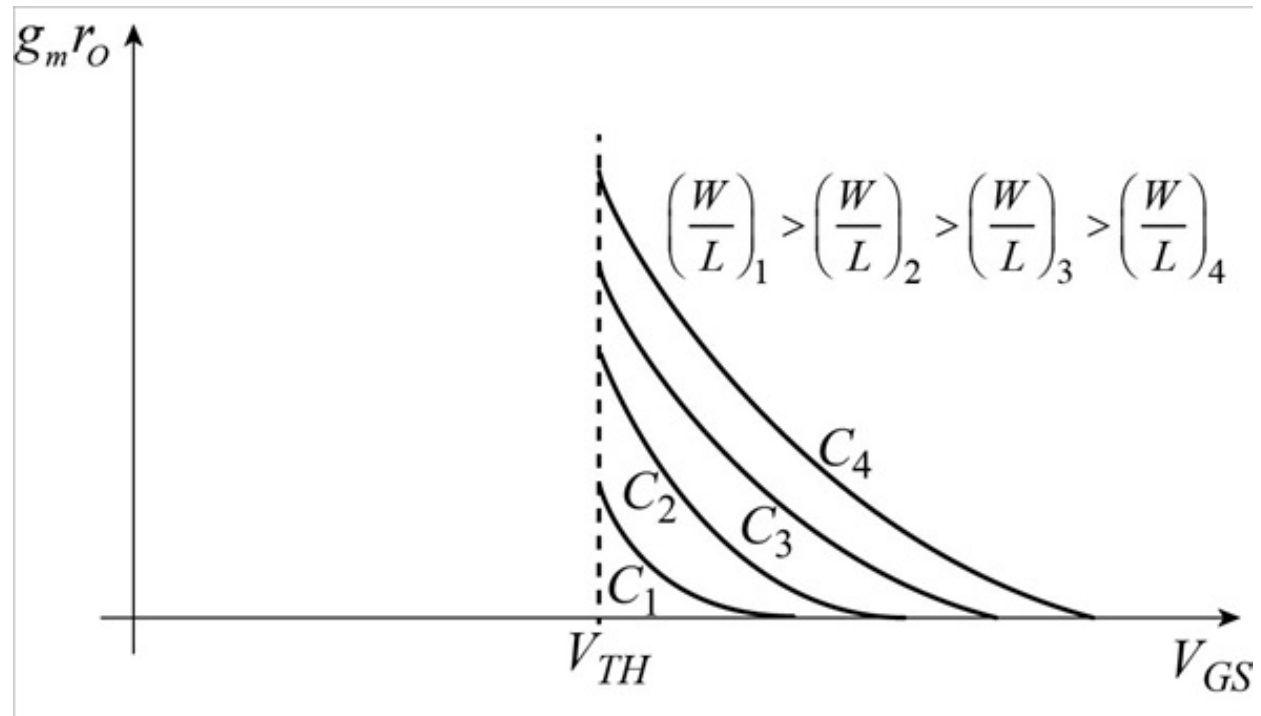
\includegraphics[width=1\linewidth]{3.6-4}
	\end{minipage}
	\caption*{图1} %最终文档中希望显示的图片标题
\end{figure}

\scalebox{3}{(b)}

		\begin{figure}[H] %H为当前位置,!htb为忽略美学标准,htbp为浮动图形
	\begin{minipage}{\linewidth}
		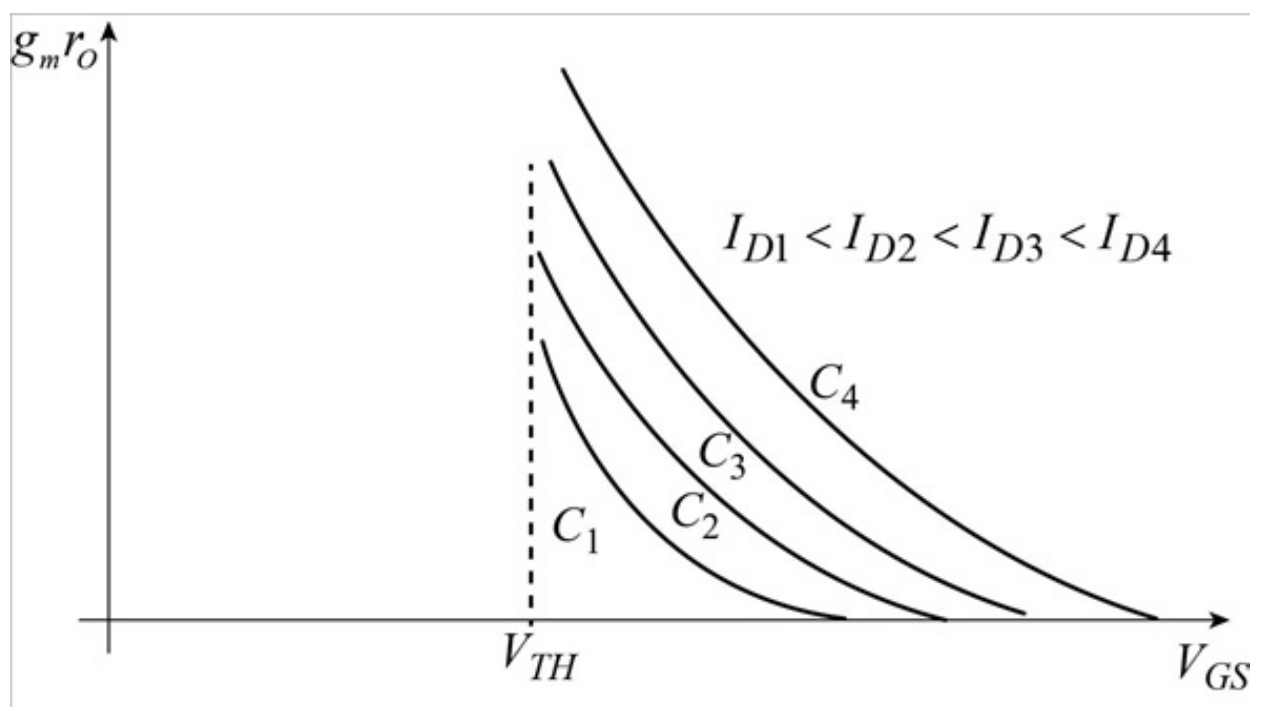
\includegraphics[width=1\linewidth]{3.6-5}
	\end{minipage}
	\caption*{图2} %最终文档中希望显示的图片标题
\end{figure}







